\graphicspath{{../Graphics/Cpt2-InjectCW/}}

En este cápitulo se ha estudiado la creación de OFC mediante inyección de luz en función de las condiciones de la inyección, dadas por la potencia inyectada $P_{Iny}$ y la diferencia de frecuencias $\delta \nu$ entre la frecuencia del láser maestro y el láser esclavo (ML y SL respectivamente por sus siglas en inglés). Se ha trabajado con el láser ML en corriente continua con $\ibias = 35$ mA, $V_{RF} = 0$ V y $f_R = 5.0$ GHz.

Se han obtenido los diferentes régimenes dinámicos de los OFC en función de $P_{Iny}$ para dos valores de $\delta\nu$ distintos, uno positivo que equivale a una frecuencia de SL menor que la de ML, y otro negativo con el caso contrario.

En la Figura \ref{Img:zonasIO} se muestran los espectros ópticos con inyecci\'on \'optica de las diferentes regiones dinámicas obtenidas para diferentes valores de $P_{Iny}$ a $\delta\nu = -2$ GHz. 

			\begin{figure}[H]
				\centering
				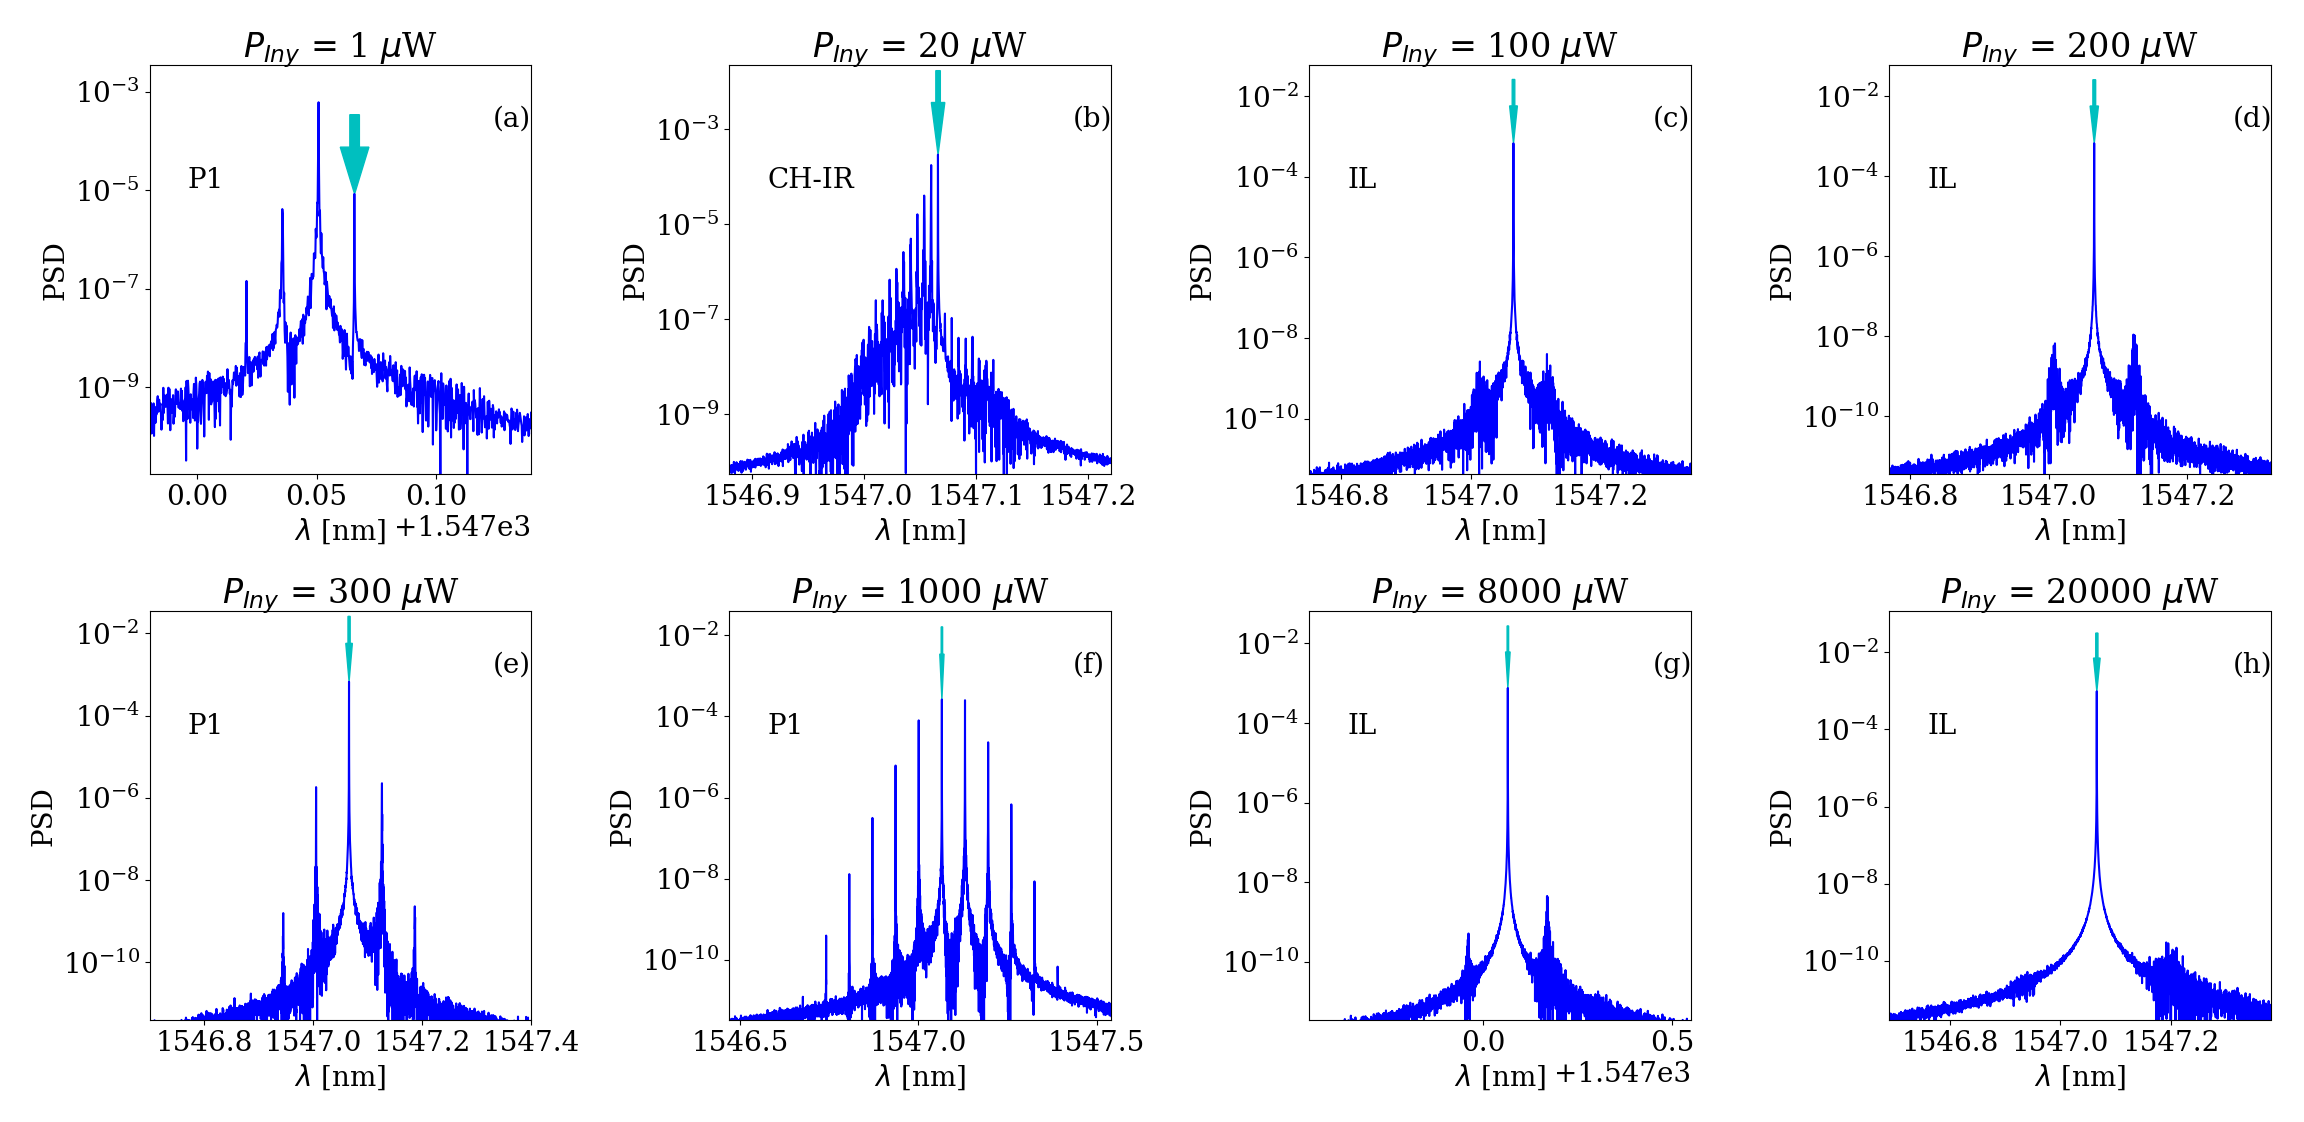
\includegraphics[width=1.0\linewidth]{zoneMap.png}
				\caption{\label{Img:zonasIO}Espectros ópticos con inyección \'optica de las diferentes regiones dinámicas obtenidas para diferentes valores de $P_{Iny}$ para $\delta\nu = -2$ GHz. Se indica la frecuencia de inyección $\nu_{SL}$ con una flecha y $P_{Iny}$ para cada espectro óptico.}
			\end{figure}

		Para una baja potencia de inyección $P_{Iny} = 1 \; \mu$W (Figura \ref{Img:zonasIO} (a)) se obtiene un espectro óptico con el pico de emisión de ML y dos picos estimulados para la frecuencia de inyección $\nu_{SL}$. En esta región denominada de periodo 1, P1, las variables internas del áser logran estabilizarse \cite{vainio2006diode} debido a un fenómeno de \textit{Four-wave mixing} (FWM, mezcla de cuatro ondas). Al aumentar $P_{Iny}$ se llega a una región de caos, CH-IR ($P_{Iny} = 20\; \mu$W, Figura \ref{Img:zonasIO} (b)), con un OFC formado por muchas líneas y con un perfil irregular. Esta región de caos se destruye para $P_{Iny} = 100\;\mu$W, en la que se obtiene un espectro óptico con una única línea de emisión para la frecuencia de inyección $\nu_{SL}$. Al aumentar la potencia de SL el láser bloque la emisión en $\nu_{ML}$ pasando a emitir solo en $\nu_{SL}$. A este fenómeno se le conoce como Bloqueo de Inyección (IL por sus siglas en inglés). En la Figura \ref{Img:zonasIO} (d) se muestra el espectro para $P_{Iny} = 200\;\mu$W en IL, observando com al aumentar la potencia de inyección se empiezan a estimular las frecuencias de las oscilaciones de relajación. Esto indíca que nos encontramos en el límite de la región IL, encontrando una bifurcación de Van't Horf. Si se continúa aumentando la potencia de inyección aumentarán los picos de la frecuencia de oscilaciones de relajación, retornando a la región P1 ($V_{RF} = 300\;\mu$W, Figura \ref{Img:zonasIO} (e)). Dentro de la refión P1, el aumento de la potencia de inyección produce la aparición de nuevas líneas de emisión, creciendo el OFC. Para altas potencias de inyección, $P_{Iny} = 8000 \;\mu$W y $20000 \;\mu$W, se regresa a la región IL.

		A partir de los datos experimentales para un láser de modo discreto en corriente continua $\ibias = 30$ mA \cite{Chaves19}, se ha obtenido un mapa con las diferentes regiones dinámicas en función de $P_{Iny}$ y $\delta\nu$. En la Figura \ref{fig:map} se muestra el mapa de las regiones dinámicas obtenido a partir de \cite{Chaves19}, marcando los putos correspondientes a los espectros ópticos de la Figura \ref{Img:zonasIO}.

			\begin{figure}[H]
				\centering
				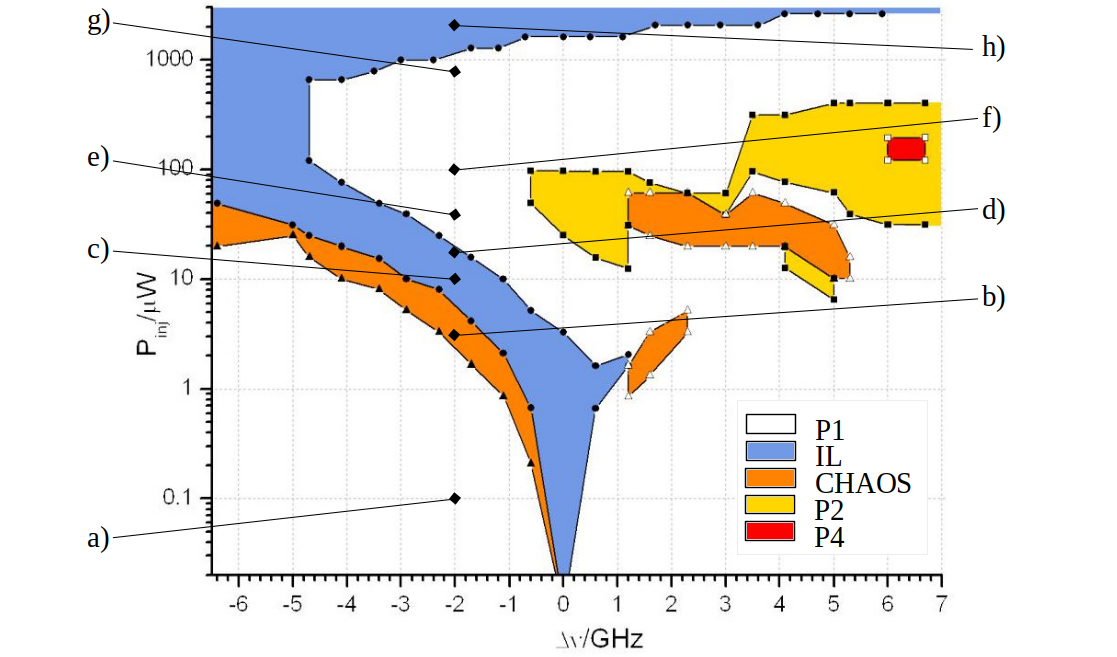
\includegraphics[width=0.7\linewidth]{maps.png}
				\caption{\label{fig:map}Mapa con las diferentes regiones dinámicas en función de $P_{Iny}$ y $\delta\nu$ obtenido a partir de \cite{Chaves19}. Se han marcando los putos correspondientes a los espectros ópticos de la Figura \ref{Img:zonasIO}.}
			\end{figure}

		Las regiones dinámicas del mapa de la Figura \ref{fig:map} obtenidas experimentalmente, para las condiciones de inyección de los espectros ópticos de la Figura \ref{Img:zonasIO} corresponden a las regiones obtenidas del análisis de los resultados de la simulación.

		En la Figura \ref{fig:zoneRtEq} se muestran la potencia $P(t)$, la fase óptica $\Phi (t)$ y el espectro óptico de los tres casos más representativos de la Figura \ref{Img:zonasIO} para cada región dinámica obtenida: CH-IR, IL y P1. Esto permite estudiar los procesos que tienen lugar en las tres regiones encontradas para $\delta\nu = -2$ GHz. 

			\begin{figure}[H]
				\centering
				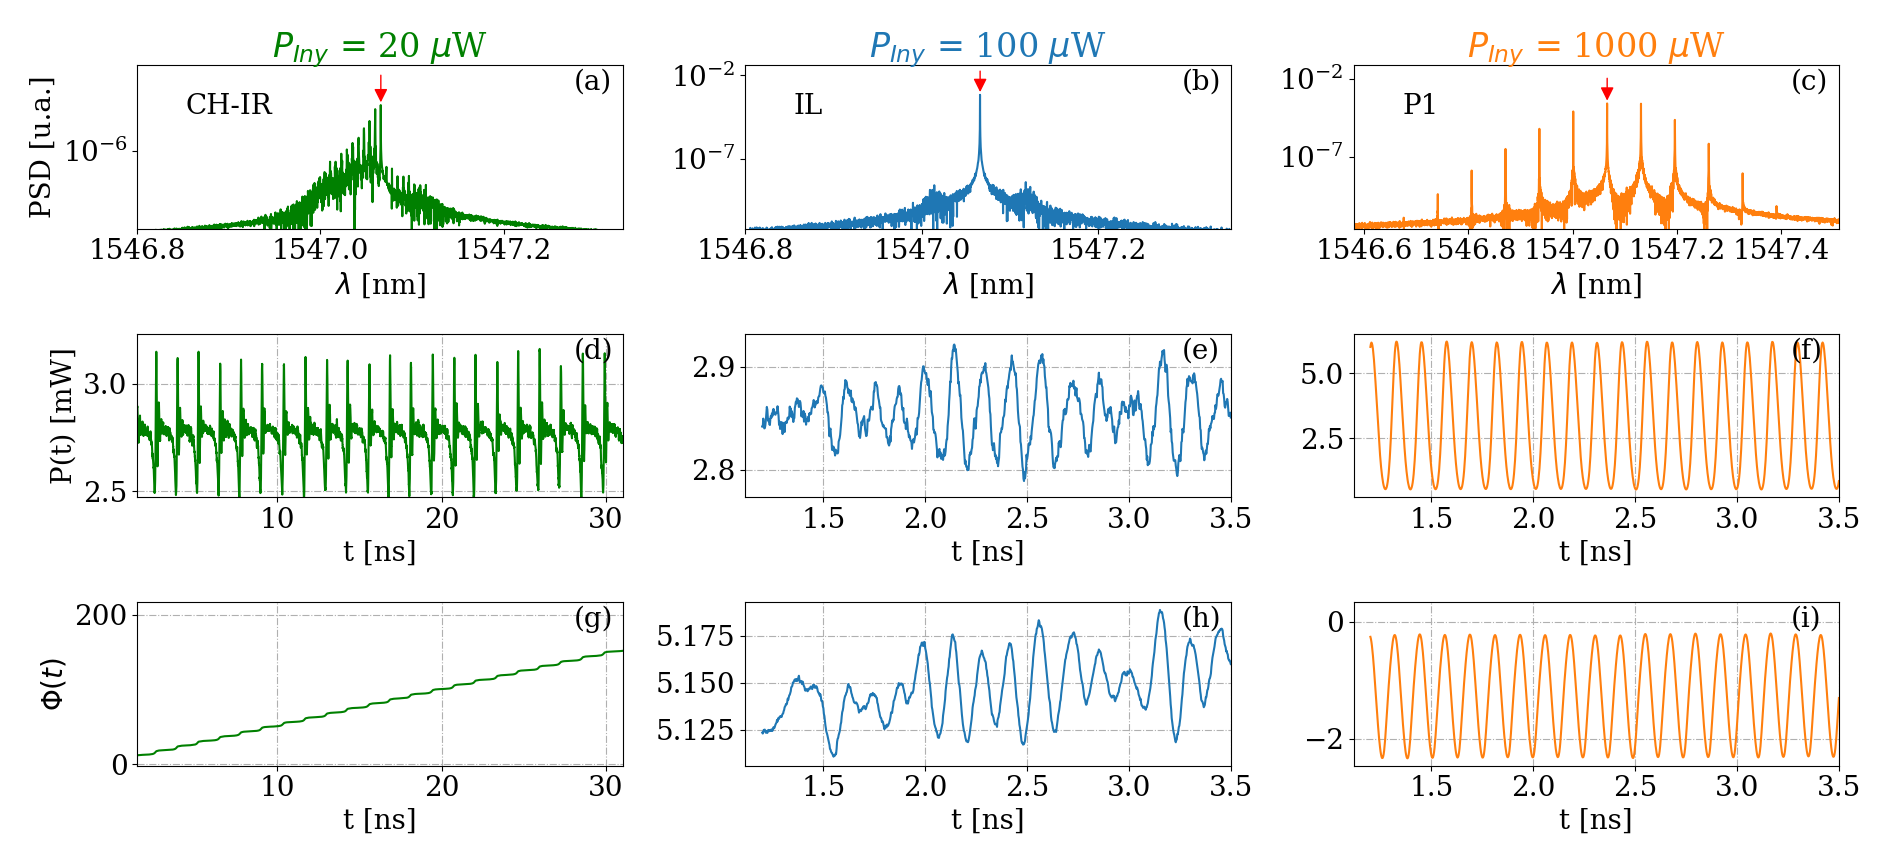
\includegraphics[width=1.0\linewidth]{zoneRtEq.png}
				\caption{\label{fig:zoneRtEq}Potencia $P(t)$, fase óptica $\Phi (t)$ y espectro óptico de los tres casos más representativos de la Figura \ref{Img:zonasIO} para cada región dinámica obtenida: CH-IR con $P_{Iny} = 20\;\mu$W (verde), IL con $P_{Iny} = 100\;\mu$W (azul) y P1 con $P_{Iny} = 1000\;\mu$W (naranja). Se indica en los espectros la frecuencia de inyección $\nu_{SL}$ con una flecha.}	
			\end{figure}

		Para el caso con $P_{Iny} = 1000\;\mu$W de la rigión P1 se obtiene un espectro óptico (Figura \ref{fig:zoneRtEq} (c)) se obtiene un OFC de buena calidad formado por varias líneas bien resueltas y con las misma serparación entre ellas. Los perfiles temporales que se obtienen para $P(t)$ y $\Phi(t)$ son oscilaciones con una amplitud y periodo bien definidos, mostrando la estabilización debida al FWM. En la Figura \ref{fig:zoneRtEq} (e)  se muestra el perfil temporal de la potencia para $P_{Iny} = 100\;\mu$W IL, que toma valores cercanos a un valor constante, realizando variaciones aleatroria y pequeñas entorno a dicho valor. Esto mismo se observa para su fase óptica (Figura \ref{fig:zoneRtEq} (h)) en la que se obtienen variaciones de $\Phi(t)$ tres ordenes de magnitud menores que para P1. Con $P_{Iny} = 20\;\mu$W se encuentra la región CH-IR, con un perfil temporal de $P(t)$ similar al de IL (Figura \ref{fig:zoneRtEq} (d)) pero con unas pequeñas oscilaciones anarmónicas en un periodo $T \approx 1.25$ ns. La fase ótica en CH-IR (Figura \ref{fig:zoneRtEq} (g)) aumenta a medida que el tiempo avanza.

		Del mapa de regiones dinámicas de la Figura \ref{fig:map} se deduce que para $\delta\nu$ positivo se ha de poder alcanzar regiones con doblamiento de periodo, P2. En la Figura \ref{fig:P2zone} se muestran los espectros ópticos, $P(t)$ y el atractor en el espacio de estados de las ecuaciones de balance, despreciando los efectos de la fase óptica; para $\delta\nu = 5$ GHz y $P_{Iny} = 50\;\mu \textrm{W, } 1000\;\mu\textrm{W y } 200\;\mu$W.

			\begin{figure}[H]
				\centering
				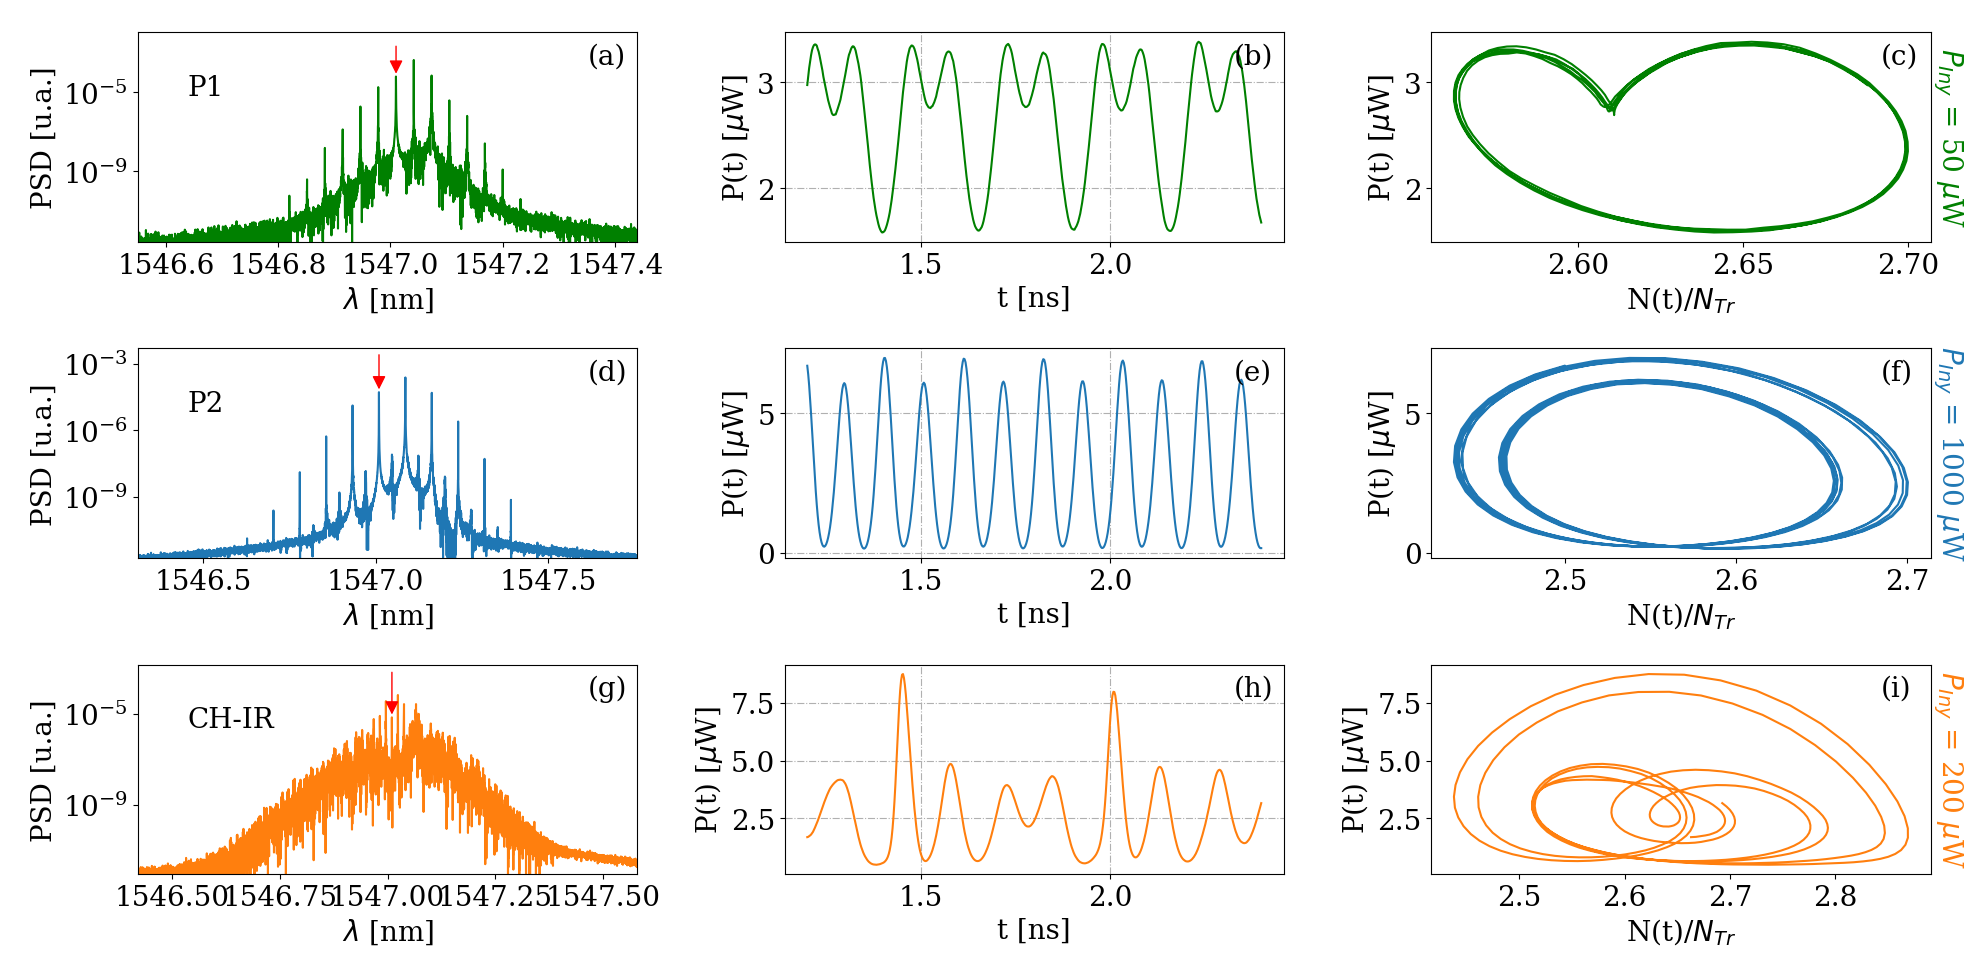
\includegraphics[width=1.0\linewidth]{P2zone.png}
				\caption{\label{fig:P2zone}Espectros ópticos, $P(t)$ y atractor en el espacio de estados de las ecuaciones de balance, despreciando los efectos de la fase óptica; para $\delta\nu = 5$ GHz y $P_{Iny} = 50\;\mu \textrm{W (verde), } 1000\;\mu\textrm{W (azul) y } 200\;\mu$W (naranja). Se indica en los espectros la frecuencia de inyección $\nu_{SL}$ con una flecha.}	
			\end{figure}

			Se obtiene de nuevo un OFC de buena calidad para la región P1 ($P_{Iny} = 50\;\mu$W, Figura \ref{fig:P2zone} (a)) y una $P(t)$ oscilante con una amplitud y frecuencia determinada (Figura \ref{fig:P2zone} (b)). Sin embargo, se observa como los máximos de $P(t)$ comienzan a desdoblarse formando una segunda oscilación, indicando que se encuentra cerca de una región con doblamiento de periodo P2. Ésto no se observa en el espectro óptico debido a la poca intensidad de estos picos y al ruido debido a la emisión espontánea, pero sí se puede ver en la Figura \ref{fig:P2zone} (c). El diagrama no llega a realizar una revolución completa sino que se dobla hacia el interior en un determinado punto. Al llegar la región P2 ($P_{Iny} = 1000\;\mu$W) la potencia se ha desdoblado completamente (Figura \ref{fig:P2zone} (e)), alternando picos de mayor y menor potencia. En el espectro óptico (Figura \ref{fig:P2zone} (d)) se obtienen líneas de emisión escitadas entre las que se teían en P1. La frecuencia de separación entre las líneas cae a la mitad $\Delta \nu' = \frac{\Delta\nu}{2}$ y así el periodo es el doble. En la Figura \ref{fig:P2zone} (f) aparece una nueva oscilación de menor amplitud debido al desdoblamiento de $P(t)$ y $N(t)$.

		Se alcanza la región CH-IR para $P_{Iny} = 200\;\mu$W, obteniendo un perfil de $P(t)$ con oscilaciones aleatrorias y sin una amplitud o frecuencia determinada (Figura \ref{fig:P2zone} (h)). El OFC del espectro óptico (Figura \ref{fig:P2zone} (g)) se destruye completamente y el diagrama de estados de la Figura \ref{fig:P2zone} (i) describe una trayectoria irregular que para rangos de tiempo suficientemente grandes cubriría todo el espacio. 

		En la Figura \ref{fig:maps2} se muestra el mapa de las regiones dinámicas obtenido a partir de \cite{Chaves19}, marcando los puntos correspondientes a las condiciones de inyección de los resultados de la Figura \ref{fig:P2zone}, obteniendo las mismas regiones que mediante el análisis de los resultados de la simulación.

			\begin{figure}[H]
				\centering
				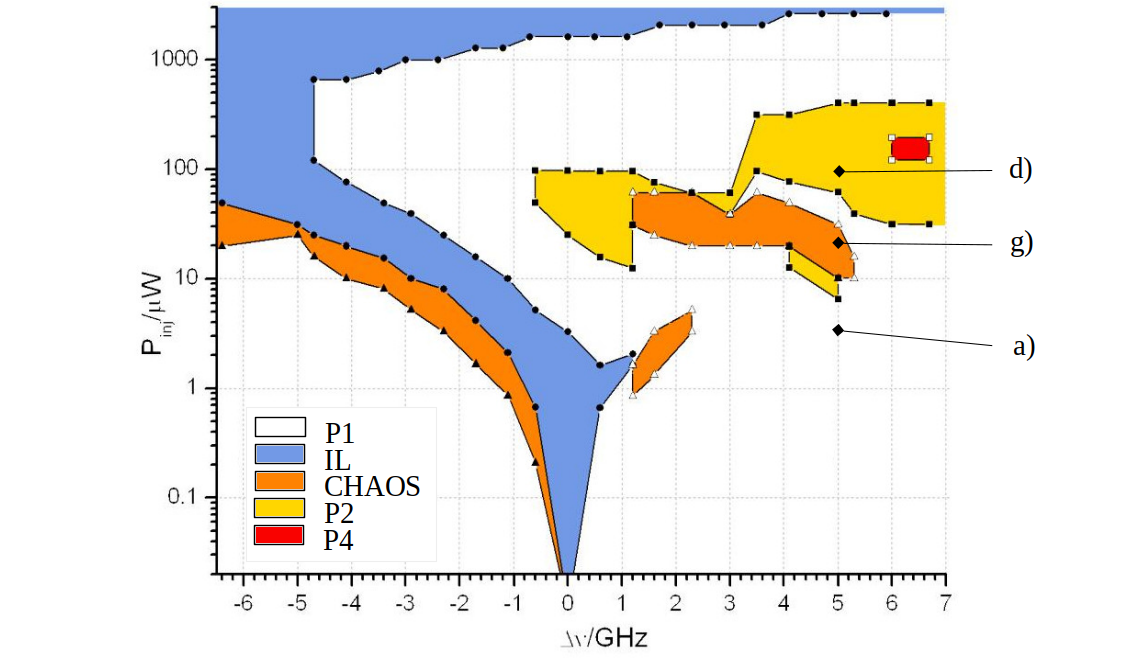
\includegraphics[width=0.7\linewidth]{maps2.png}
				\caption{\label{fig:maps2}Mapa con las diferentes regiones dinámicas en función de $P_{Iny}$ y $\delta\nu$ obtenido a partir de \cite{Chaves19}. Se han marcando los putos correspondientes a las condiciones de inyección de la Figura \ref{fig:P2zone}.}	
			\end{figure}
